%[prl] it will mess up section numbers but puts our emails in the bibliography section
%[eqsecnum] Number equations by section
%
%
%\documentclass[prd,preprint,letterpaper]{revtex4}
\documentclass[aps,prb,twocolumn,superscriptaddress]{revtex4-1}

\usepackage{graphicx}  % this is the up-to-date package for all figures
\usepackage{amssymb}   % for math
\usepackage{verbatim}  % for the comment environment
\usepackage{color}
\usepackage{subcaption} % for sub-captions on side-by-side figures
\usepackage{float}	% allows use of 'H' command
\usepackage{tikz} % lets you draw: graphics, flowcharts, pie graphs, etc

%%%
% For fancy section references
%%% 
% This allows you to use '\cref{}' to reference sections with the symbol
\usepackage{cleveref}
\crefname{section}{\S}{\S\S}%{§}{§§}
%% Usual (decimal) numbering
\renewcommand{\thesection}{\arabic{section}}
\renewcommand{\thesubsection}{\thesection.\arabic{subsection}}
\renewcommand{\thesubsubsection}{\thesubsection.\arabic{subsubsection}}
%% Fix references
\makeatletter
\renewcommand{\p@subsection}{}
\renewcommand{\p@subsubsection}{}
\makeatother
%%%%%
%%%


\def\deg{\ifmmode^\circ\else$^\circ$\fi}
\def\arcsec{\ifmmode^{\prime\prime}\else$^{\prime\prime}$\fi}
\def\arcmin{\ifmmode^{\prime}\else$^{\prime}$\fi}
\def\solar{\ifmmode_{\mathord\odot}\else$_{\mathord\odot}$\fi}
\def\earth{\ifmmode_{\mathord\oplus}\else$_{\mathord\oplus}$\fi}

%%%
% Change labeling of figures and tables - currently it defaults to 'FIG.'
%%%
\renewcommand{\figurename}{Figure}
\renewcommand{\thefootnote}{\roman{footnote}} %for footnotes in roman numerals
%\renewcommand{\thetable}{\Roman{table}}

\bibliographystyle{apsrev}


% these are some custom control of the page size and margins
% \topmargin= 0.2in  % these 1st two may be needed for some computers
% \textheight=8.75in
\textwidth=6.5in
%\oddsidemargin=0cm
%\evensidemargin=0cm


\begin{document}

\title{Assassinating ASASSN: Supernovae Identification Using ATLAS Data}

\author{Corey Mutnik}
\email{cmutnik@hawaii.edu}
\affiliation{Department of Physics \& Astronomy, \\
University of Hawaii at Manoa,\\
2505 Correa Rd, Honolulu, HI, 96822, USA}
\altaffiliation{ASTR 399}



% \section is used to start a new one with a heading
\begin{abstract}
Using current data collection and reduction techniques, we plan to 
identify SN faster and fainter than the All-Sky Automated Survey for Supernovae (ASASSN) team is able to. 
%With a declination limit of $-30^{\circ}$
We expect to identify all supernovae (SNe), with $m>17.5$ and declinations above $-30\deg$, 
before ASASSN is able to.\\
%We expect to identify all supernovae (SN) above a declination of $-30\deg$, with $m>17.5$, before ASASSN is able to.\\
{\bf 17.5 (0.5mag) --OR-- 18 (1mag) fainter...which is it?}\\
{\bf not emphasis on Type Ia supernovae}
\end{abstract}


\maketitle    



\section{Introduction}
Supernovae (SN) identification using data collected by ATLAS.

{\bf fix biblio style / numbering}
{\bf Look at previous JT paper to see if:\\
numbers inside mathmode: -30$^{\circ}$, $-30^{\circ}$\\
abbreviations in abstract: ... (ASASSN), or is just ASASSN good\\
}

{\bf check plurality throughout paper, SN or SNe}

%\section{Data}

%\section{ASASSN Breakdown}
\section{ASASSN Data}
\begin{itemize}
	\item{} Where'd it come from
	\item{} ASASSN specs
\end{itemize}


\indent The All-Sky Automated Survey for Supernovae (ASASSN) group 
collects data using two $14~cm$ telescopes. Each night these two 
telescopes are able to cover roughly $20,000~deg^{2}$ and reach 17th magnitude.
{\bf reword}\\
The first telescope is located on Haleakala and began collecting data December 
2013. In July 2015 a second telescope became operational at the LCOGT 
Cerro Tololo station. {\bf Cite using footnote.}
%~\footnote{http://www.astronomy.ohio-state.edu/~assassin/index.shtml}


%data collected by two 14--cm telescopes\\
%one at Haleakala, the other at the LCOGT Cerro Tololo station.\\
%first guy started in December 2013...second came online in July 2015.\\
%these two currently cover roughly 20,000~$deg^{2}$ a night\\
%down to 17th mag\\
%they eventually plan to survey the entire sky, every night, down to 17th mag, using 16 scopes at 4 diff sites\\
%\footnote{http://www.astronomy.ohio-state.edu/~assassin/index.shtml}

{\bf Fix citations: ASASSN data~\cite{asn_data} or use diff cite method\\
\citet{asn_data}\\
\citealt{asn_data}\\
...Should be ``Shappee et al. (2014)''
}

% OLD plots as single
 %\begin{figure}[H]%[h!]
 %  \begin{center}
 %\centerline{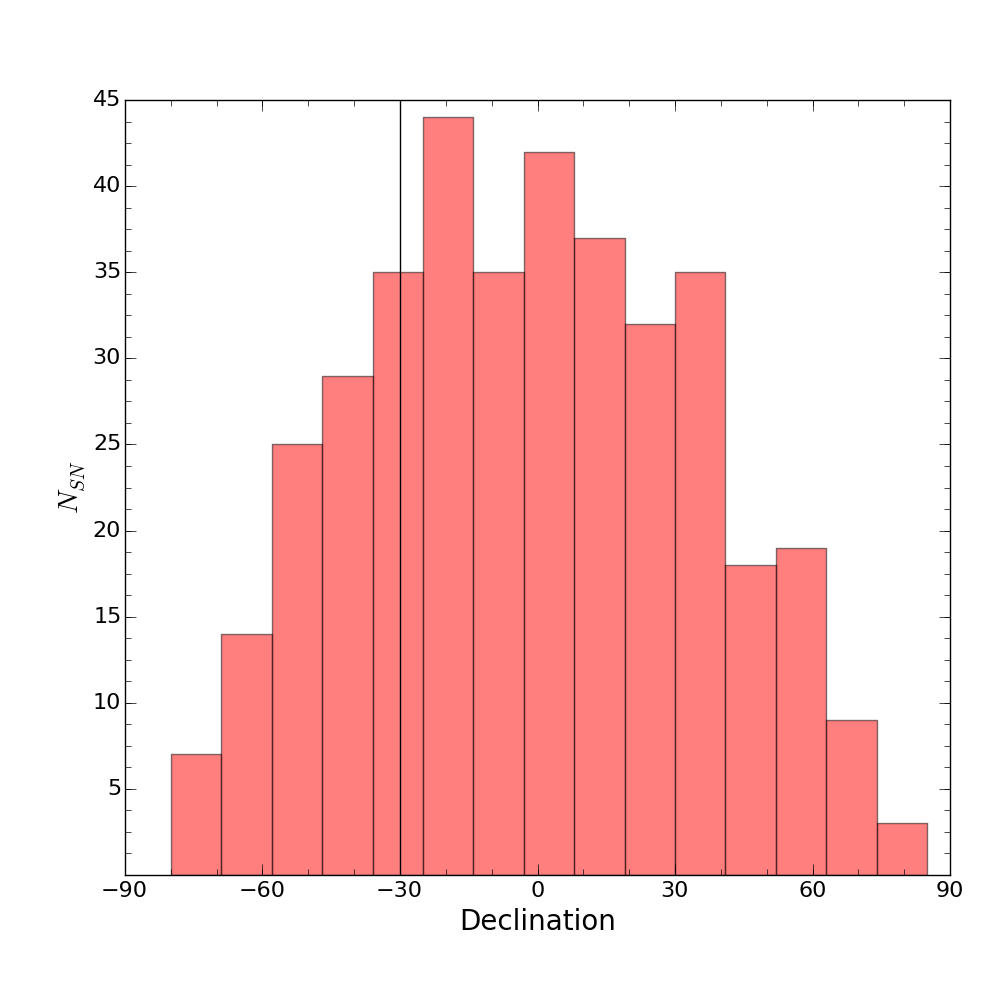
\includegraphics[width=3.35in]{figures/dec_histo_step10.png}}
 %\caption{\it \small{ASASSN SN sorted by their declination. The vertical line at $-30^{\circ}$ indicates the lower limit on ATLAS observations. \label{fig:asn_dec}}}
 %  \end{center}
 %\end{figure}
 %\begin{figure}[H]%[h!]
 %  \begin{center}
 %\centerline{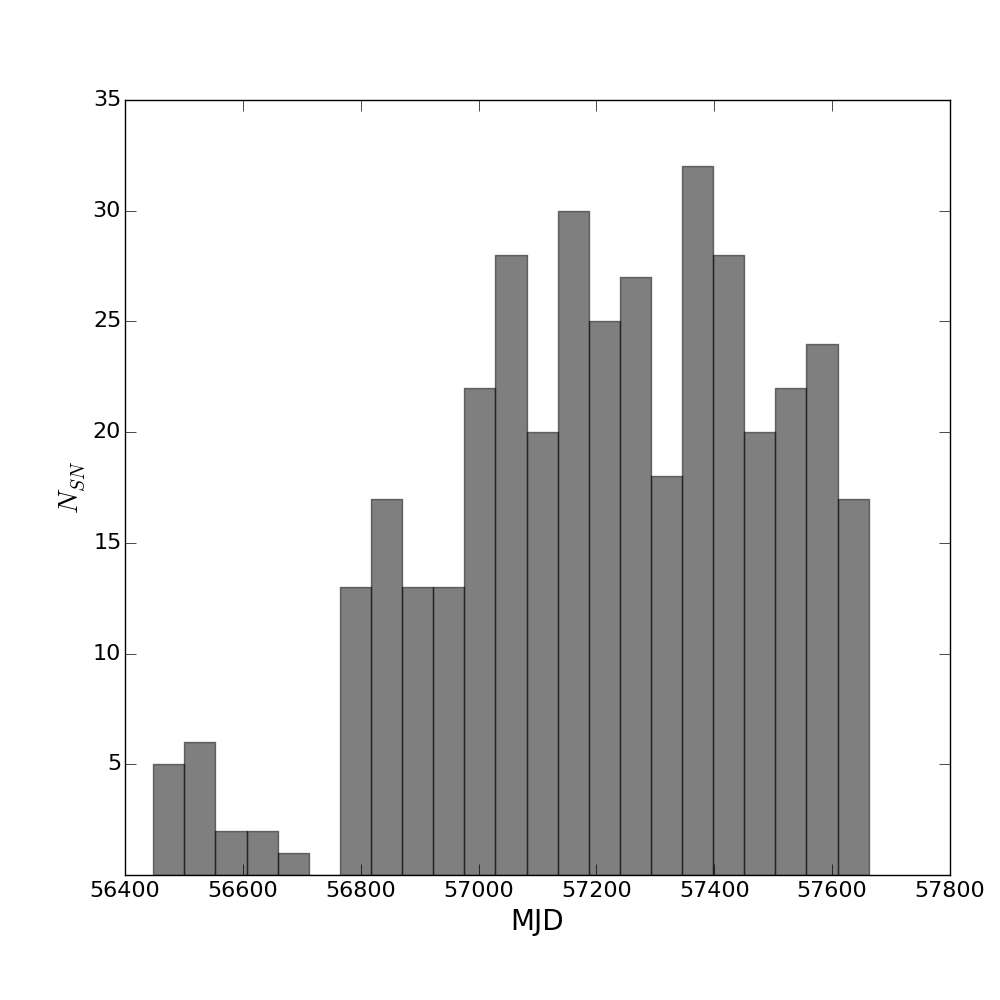
\includegraphics[width=3.35in]{figures/mjd_histo_step50.png}}
 %\caption{\it \small{Discovery date of ASASSN SN. \label{fig:asn_mjd}}}
 %  \end{center}
 %\end{figure}
 %~[MAKE THIS A DUAL FIGURE: (a) (b)]
~\\~{\bf [REBIN MJD DATA FOR PEAK BRIGHTNESS DATE NOT DISCOVERY DATE]}\\
{\bf Need to reference Figure~\ref{fig:asnhist} --OR-- Figures~\ref{fig:mjdhist}~and~\ref{fig:dechist}}

\begin{figure*}
	\centering
	\begin{subfigure}{.5\textwidth}
	  \centering
	  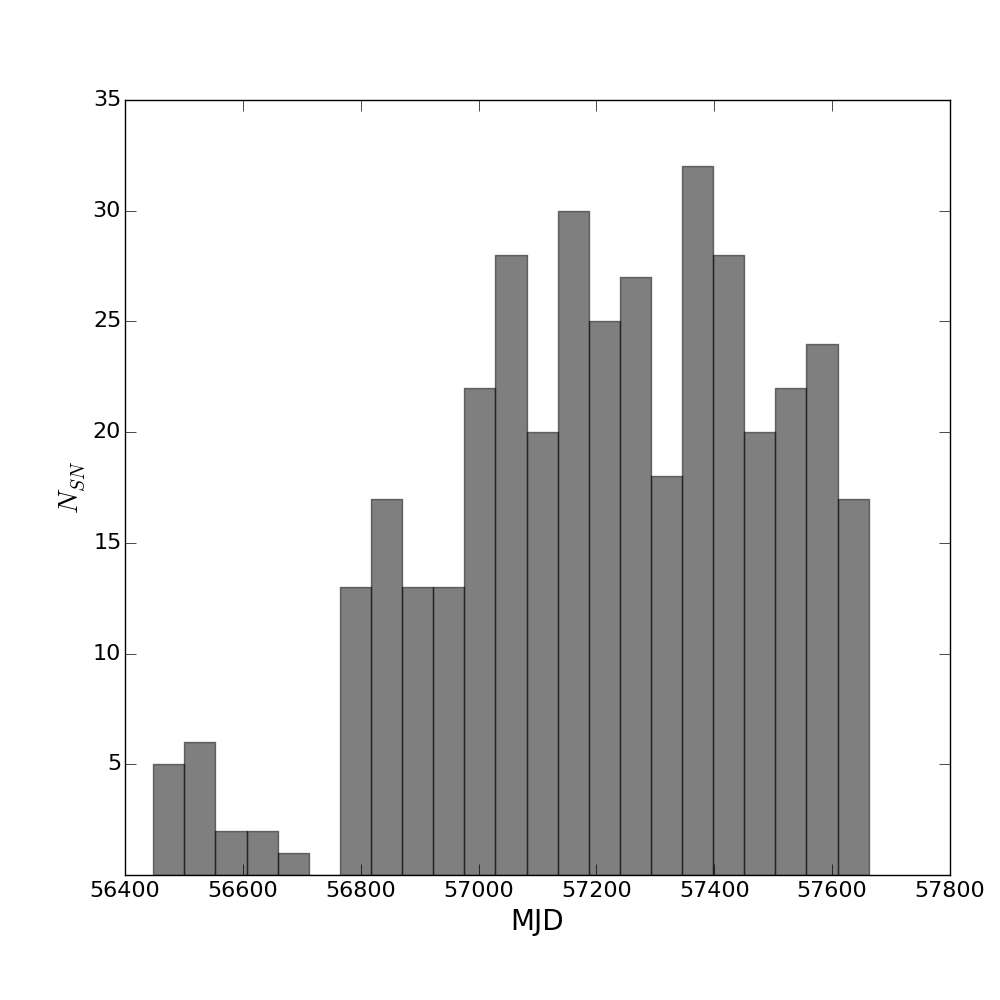
\includegraphics[width=1\linewidth]{figures/mjd_histo_step50.png}
		\caption{\it \small{ }}
		\label{fig:mjdhist}
	\end{subfigure}%
	\begin{subfigure}{.5\textwidth}
	  \centering
			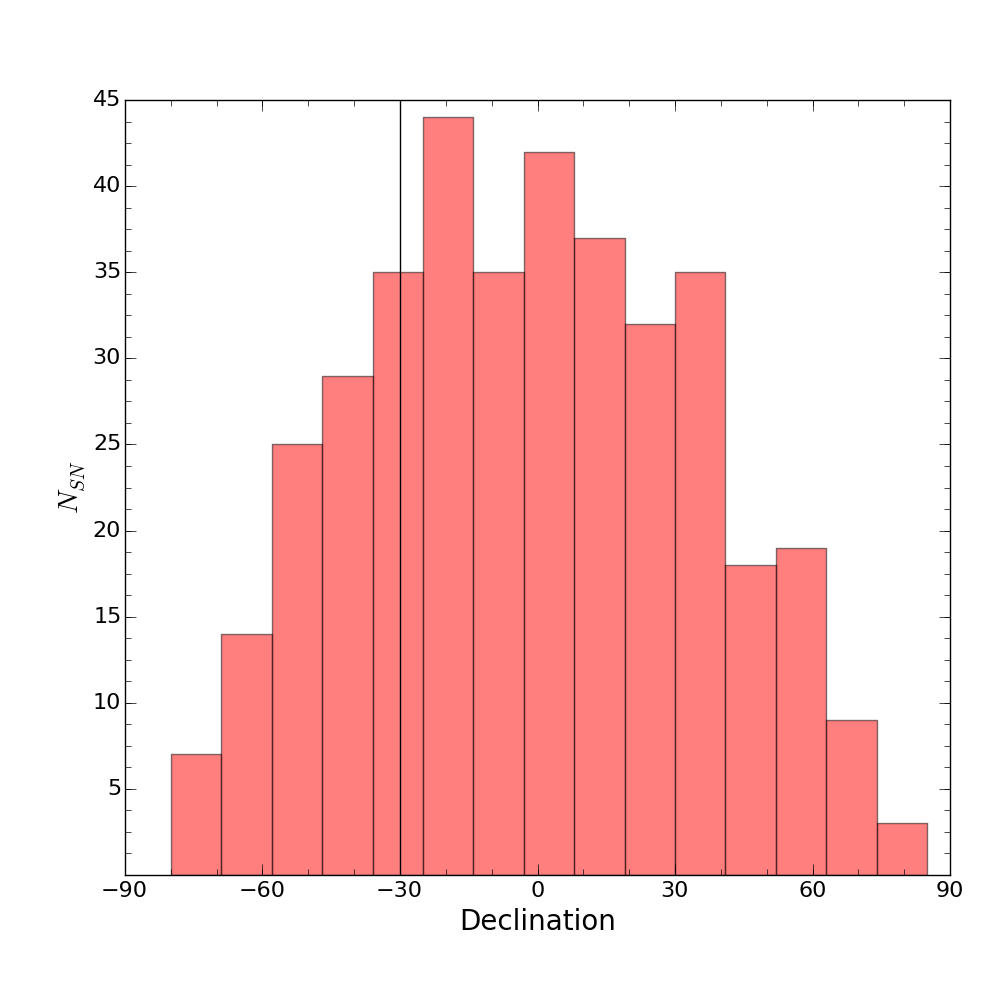
\includegraphics[width=1\linewidth]{figures/dec_histo_step10.png}
		\caption{\it \small{ }}
		\label{fig:dechist}
	\end{subfigure}
	\caption{\it \small{SN discovered by the ASASSN project.  Panel `(a)' shows ASASSN SN discovery dates.  Panel `(b)' is ASASSN data, binned by dec. The vertical line at $-30^{\circ}$ indicates the lower limit on ATLAS observations.}}
	\label{fig:asnhist}
\end{figure*}


\section{ATLAS PathFinder 2 Observations}
\begin{itemize}
	\item{} ATLAS specs
	\item{} how data was collected
	\item{} how *.diff.fz is made - subtract wallpaper from reduced data
	\item{} how *.ddt is made
	\item{} what is starrat
\end{itemize}



\section{Procedure}
\begin{enumerate}
	\item{} find asn SN in atlas data
	\item{} use asn SN to restrict ATLAS classification variables
	\item{} manually inspect results for SN classification
\end{enumerate}
{\bf want to make input sections subsections under this section?}
%%%
% input 2 sections: ``Expected Observations'' and ``Failed Matches''
%%%
\input section_expected_obs.tex




\section{SN Identification}
How ASASSN SN help identify those in ATLAS data.




\section{Results and Discussion}
\begin{enumerate}
	\item{} what restrictions we intend to place on things like starrat
	\item{} 
\end{enumerate}

\newpage\newpage
%\clearpage








\section*{Acknowledgments}
I would like to thank \input acknowledgement.tex  % input acknowledgement



\setlength{\parindent}{0cm}

\bibliography{biblio}

%\begin{thebibliography}{99}  % the trailing 99 controls some obscure format--just use
%\bibitem{Sch_eq} Weisstein, Eric W. ``Schr\"{o}dinger Equation."
%{\em Schr\"{o}dinger Equation. } Mathematica, 1996. Web. 2 May 2015.
%\end{thebibliography}

\end{document}
